\documentclass{beamer}
\usepackage{amsmath}
\usepackage{amssymb}
\usepackage{graphicx}
\usepackage{babel}
\usepackage{tikz}
\usepackage{listings}
\lstset{
    basicstyle=\tiny,
    language=caml
}
% AMS Packages
\usepackage{amsmath}
\usepackage{amsthm}
\usepackage{amssymb}

% Unicode
\usepackage[utf8]{inputenc}


\usetikzlibrary{arrows.meta}
\newcommand {\axes}[4] {\draw[->] (0,0) -- (#3,0) node [right]{#1};
                        \draw[->] (0,0) -- (0,#4) node[above]{#2};}
\newcommand {\valx}[2] {\draw (#1,0.03) -- (#1,-0.03) node[anchor=north]{#2};}
\newcommand {\valy}[2] {\draw (0.03,#1) -- (-0.03,#1) node[anchor=east]{#2};}




\title{TIPE Sur l'optimisation du trafic routier.}
\author{DURAND Ulysse}
\everymath{\displaystyle}




% \usetheme{Madrid}

\usecolortheme{seahorse}
\useoutertheme{infolines}
\setbeamerfont{block title}{size={}}
\setbeamercolor{titlelike}{parent=structure,bg=white}

\date{2020-2021}
\institute{MPX-Lycée Blaise Pascal}
\begin{document}
\maketitle


\begin{frame}
\frametitle{Sommaire}
\begin{enumerate}
    \item Enoncé du problème
    \item Modélisation - structure de donnée
    \item Résolution approchée : se rammener à minimiser une fonction
    \item Résolution dans un cas particulier : les graphes série parallèle
\end{enumerate}
\end{frame}

\begin{frame}
\frametitle{Le problème}
On souhaite fluidifier un trafic routier
\begin{itemize}
\item On a un certain débit de voitures à acheminer d'un point A à un point B
\item On peut agir sur le chemin pris par les voitures
\item On souhaite réduire le temps de trajet moyen des voitures
\item Plus le déit de voitures sur une route est important plus le temps
nécessaire pour parcourir la route est élevé
\item 
\end{itemize}
\end{frame}

\begin{frame}
\frametitle{Modèle - Structure de donnée}
\begin{itemize}
\item Le réseau routier : un graphe orienté pondéré.
\item Une route : une arète
\item Une intersection : un noeud
\item Modèle de ralentissement : une fonction du temps de parcours de la route en 
fonction du débit sur la route. (fonction de ralentissement)
\end{itemize}
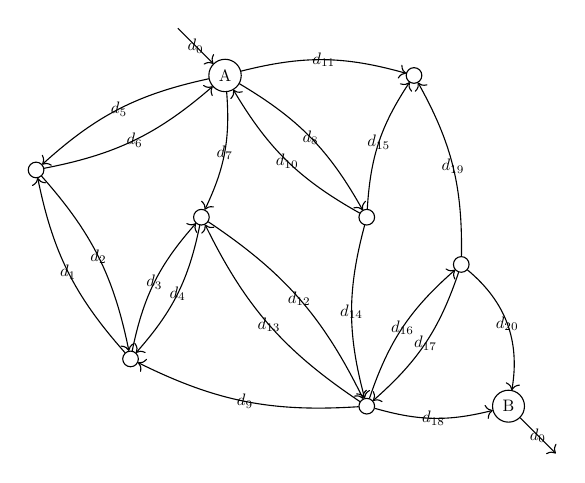
\begin{tikzpicture}[scale = 0.6, every node/.style={scale=0.6}]
    \node[shape=circle,draw=black] (A) at (3,3) {};
    \node[shape=circle,draw=black] (B) at (1,7) {};
    \node[shape=circle,draw=black] (C) at (5,9) {A};
    \node[shape=circle,draw=black] (D) at (4.5,6) {};
    \node[shape=circle,draw=black] (E) at (8,2) {};
    \node[shape=circle,draw=black] (F) at (8,6) {};
    \node[shape=circle,draw=black] (G) at (9,9) {};
    \node[shape=circle,draw=black] (H) at (10,5) {};
    \node[shape=circle,draw=black] (I) at (11,2) {B};
    \draw [->](4,10) -- node{$d_0$} (C);
    \draw [->](A) to[bend left=15] node {$d_1$} (B);
    \draw [->](B) to[bend left=15] node {$d_2$} (A);
    \draw [->](A) to[bend left=15] node {$d_3$} (D);
    \draw [->](D) to[bend left=15] node {$d_4$} (A);
    \draw [->](C) to[bend right=15] node {$d_5$} (B);
    \draw [->](B) to[bend right=15] node {$d_6$} (C);
    \draw [->](C) to[bend left=15] node {$d_7$} (D);
    \draw [->](C) to[bend left=15] node {$d_8$} (F);
    \draw [->](E) to[bend left=15] node {$d_9$} (A);
    \draw [->](F) to[bend left=15] node {$d_{10}$} (C);
    \draw [->](C) to[bend left=15] node {$d_{11}$} (G);
    \draw [->](D) to[bend left=15] node {$d_{12}$} (E);
    \draw [->](E) to[bend left=15] node {$d_{13}$} (D);
    \draw [->](F) to[bend right=15] node {$d_{14}$} (E);
    \draw [->](F) to[bend left=15] node {$d_{15}$} (G);
    \draw [->](E) to[bend left=15] node {$d_{16}$} (H);
    \draw [->](H) to[bend left=15] node {$d_{17}$} (E);
    \draw [->](E) to[bend right=15] node {$d_{18}$} (I);
    \draw [->](H) to[bend right=15] node {$d_{19}$} (G);
    \draw [->](H) to[bend left=30] node {$d_{20}$} (I);
    \draw [->](I) -- node{$d_0$} (12,1);
\end{tikzpicture}
\end{frame}

\begin{frame}
    \frametitle{Quelques fonctions de ralentissement}
    \begin{tikzpicture}[scale=3, every node/.style={scale=0.5}]
        \axes{d}{t}{1}{0.6}
        \valx{0.9}{$d_{max}$}
        \valy{0.5}{$t_{max}$}
        \draw[{}-{Arc Barb [reversed]},line width = 0.3mm, color=red] (0,0.5)
                 -- (0.9,0.5);
    \end{tikzpicture}
    %%%%%
    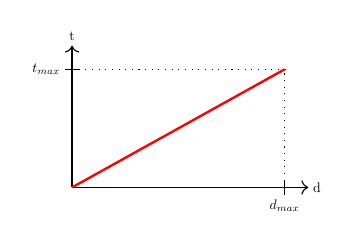
\begin{tikzpicture}[scale=3, every node/.style={scale=0.5}]
        \axes{d}{t}{1}{0.6};
        \valx{0.9}{$d_{max}$};
        \valy{0.5}{$t_{max}$};
        \draw[line width = 0.3mm, color=red] (0,0)--(0.9,0.5);
        \draw[dotted] (0.9,0) -- (0.9,0.5);
        \draw[dotted] (0,0.5) -- (0.9,0.5);
    \end{tikzpicture}
    %%%%%
    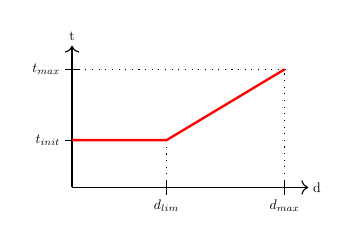
\begin{tikzpicture}[scale=3, every node/.style={scale=0.5}]
        \axes{d}{t}{1}{0.6}
        \valx{0.9}{$d_{max}$}
        \valx{0.4}{$d_{lim}$}
        \valy{0.2}{$t_{init}$}
        \valy{0.5}{$t_{max}$}
        \draw[dotted] (0.4,0.2) -- (0.4,0);
        \draw[line width = 0.3mm, color=red] (0,0.2)--(0.4,0.2) -- (0.9,0.5);
        \draw[dotted] (0,0.5) -- (0.9,0.5);
        \draw[dotted] (0.9,0) -- (0.9,0.5);
    \end{tikzpicture}
\end{frame}

\begin{frame}
\frametitle{Expression du temps de parcours moyen total}
\fontsize{8}{6}\selectfont
Du noeud A au noeud B il y a n chemins, $c_1,...,c_n$\\
Le flux total, de 1, est répartit en flux sur chaque chemin ($d_1,d_2,...,d_n$
avec $\sum_{i=1}^n d_i=1$)\\
$f_i$ la fonction de ralentissement de la route $r_i$
Les arètes disposent aussi d'un débit passant ($D_1,...,D_m$ tels que
$D_k = \sum_{i / r_k\in c_i} d_i$)\\
$t_i$ : temps de parcours du chemin i\\
Le temps de parcours moyen du graphe est la moyenne pondérée du temps de
parcours de chaque chemin par le débit du chemin.\\
$T_{tot}=\sum_{i=0}^n d_i t_i$ et
$t_i = \sum_{k/r_k\in c_i} f_k(D_k)$ \\
Intoduisons $\xi_{i,k} = 1$ si l'arrête k appartient au chemin i et 0 sinon.\\
$D_k = \sum_{i=0}^n \xi_{i,k} d_i$ et
$t_i = \sum_{k=0}^m \xi_{i,k} f_k(D_k)$\\
On a finalement l'expression de la fonction $T_{tot}$ qui a n-1 variables
$d_1,...,d_{n-1}$ ($d_n = 1-\sum_{i=0}^n d_i$)
dont on tentera d'approcher le minimum.\\
$T_{tot}=\sum_{i=0}^n d_i \sum_{k=0}^m \xi_{i,k} f_k(\sum_{i=0}^n \xi_{i,k} d_i)$\\
\end{frame}

\begin{frame}[fragile]
    \frametitle{Graphes serie parallele}

    \subsection{graphes série/parallèle}
    Un graphe série-parallèle est construit récursivement,
    de la manière suivante :\\
    C'est soit\\
    -une simple route
    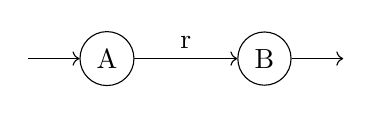
\begin{tikzpicture}[baseline=(current bounding box.center)]
        \node[shape=circle,draw=black] (A) at (0,0) {A};
        \node[shape=circle,draw=black] (B) at (2,0) {B};
        \draw [->] (-1,0) -- (A);
        \draw [->] (A) -- node[above]{r} (B);
        \draw [->] (B) -- (3,0);
    \end{tikzpicture}\\
    -deux sous graphes en parallèle
    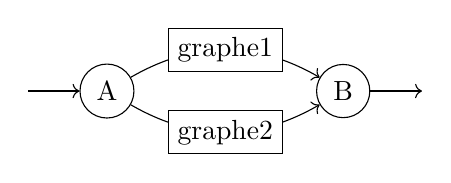
\begin{tikzpicture}[baseline=(current bounding box.center)]
        \node[shape=circle,draw=black] (A) at (0,0) {A};
        \node[shape=circle,draw=black] (B) at (3,0) {B};
        \draw [->] (-1,0) -- (A);
        \draw [->] (A) to[bend left] node[midway,draw,fill=white]{graphe1} (B);
        \draw [->] (A) to[bend right] node[midway,draw,fill=white]{graphe2} (B);
        \draw [->] (B) -- (4,0);
    \end{tikzpicture}\\
    -deux sous graphes en série
    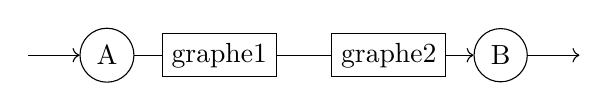
\begin{tikzpicture}[baseline=(current bounding box.center)]
        \node[shape=circle,draw=black] (A) at (0,0) {A};
        \node[shape=circle,draw=black] (B) at (5,0) {B};
        \draw [->] (-1,0) -- (A);
        \draw [->] (A) -- node[pos=0.25,draw,fill=white]{graphe1}
                            node[pos=0.75,draw,fill=white]{graphe2} (B);
        \draw [->] (B) -- (6,0);
    \end{tikzpicture}
    En ocaml : 
    \begin{lstlisting}
        type graph_ser_paral =
             Route of arrete
            |Parallel of (graph_ser_paral*graph_ser_paral)
            |Serie of (graph_ser_paral*graph_ser_paral);;
    \end{lstlisting}
\end{frame}
\begin{frame}
    \frametitle{Resolution sur graphe serie parallele}
    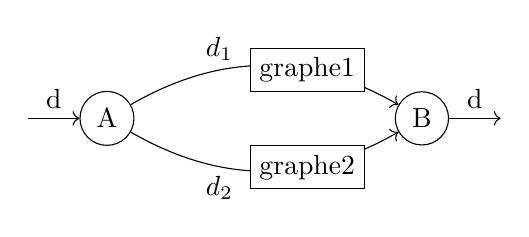
\begin{tikzpicture}[baseline=(current bounding box.center)]
        \node[shape=circle,draw=black] (A) at (0,0) {A};
        \node[shape=circle,draw=black] (B) at (4,0) {B};
        \draw [->] (-1,0) -- node[above]{d} (A);
        \draw [->] (A) to[bend left] node[pos=0.33,above]{$d_1$}
                        node[pos=0.66,draw,fill=white]{graphe1} (B);
        \draw [->] (A) to[bend right] node[pos=0.33,below]{$d_2$}
                        node[pos=0.66,draw,fill=white]{graphe2} (B);
        \draw [->] (B) -- node[above]{d} (5,0);
    \end{tikzpicture}\\
    $f_1$, $f_2$ : fonctions de ralentissement des graphes 1, 2.\\
    $\widetilde{F}(d,d_1) = \frac{d_1}{d}f_1(d_1)+\frac{d-d_1}{d}f_2(d-d_1)$ : expression du ralentissement 
    du graphe total.\\
    $\frac{\partial \widetilde{F}}{\partial d_1}(d,d_1) = \frac{1}{d}(f_1(d_1) + d_1 f_1'(d_1) - f_2(d-d_1) + (d-d_1)f'_2(d-d_1)$
    : utile pour trouver le minimum de $\widetilde{F}$\\
    En appliquant un algorithme de minimisation de fonction, on trouve $d_s$ qui
    minimise $\widetilde{F}$\\
    On obtient $F(d)=f_1(d_s(d))+f_2(d-d_s(d))$ la fonction du ralentissement du
    graphe total et $d_s(d)$ le dACCebit a diriger sur le graphe1\\
\end{frame}

\end{document}
